\chapter{Angulitos}

\section{Conceptos Básicos}

La suma de todos los ángulos alrededor de un punto siempre es 
$360\dg$. De ahí se desprende:

La suma de todos los ángulos sobre una línea recta siempre es 
$180\dg$.

Deriva que dos ángulos opuestos por el vértice son iguales 
entre si.

\begin{definition}[Ángulos suplementarios]
    Dos ángulos son sumplementarios si suman $180\dg$
\end{definition}

\begin{definition}[Ángulos complementarios]
    Dos ángulos son complementarios si suman $90\dg$
\end{definition}

\begin{definition}[Rectas perpendiculares]
    Dos rectas $l$, $m$ son perpendiculares si al intersecarse 
    forman $4$ ángulos de $90\dg$.
\end{definition}

\begin{definition}[Rectas paralelas]
    Dos rectas $l$, $m$ son paralelas si jamás se intersecan.
\end{definition}

\begin{definition}[Tangencia]
    Dos figuras son tangentes si solo tienen un punto en común.
\end{definition}


\subsection{Ángulos entre paralelas}

Supongamos que existe una línea que corta al par de rectas paralelas 
$l$ y $m$. Los ángulos que se forman mantienen las siguientes relaciones:

\begin{figure}[h]
    \centering
    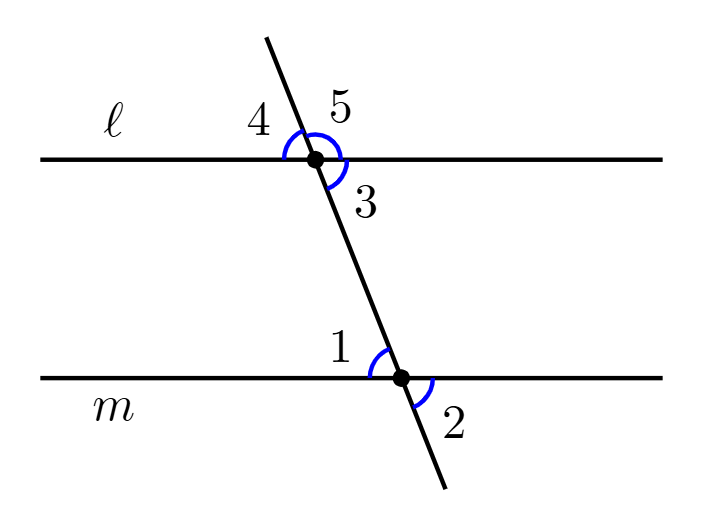
\includegraphics[height=6cm]{anglesinp.png}
\end{figure}

\begin{enumerate}[(a)]
    \item $\angle 1 = \angle 2$ y son ángulos opuestos por el vértice; 
    \item $\angle 1 = \angle 3$ y se llaman ángulos alternos internos;
    \item $\angle 1 = \angle 4$ y se llaman ángulos correspondientes;
    \item $\angle 2 = \angle 4$ y se llaman alternos internos.
\end{enumerate}

Es importante recordar que también funciona a la inversa; si se 
cumple alguna de las relaciones de ángulos de $(b)$, $(c)$ o $(d)$, 
¡las rectas serán paralelas!

\begin{theorem}
    La suma de los ángulos internos de un triángulo es $180\dg$.
\end{theorem}

\begin{proof}
    Para cualquier $\triangle ABC$, se traza una línea paralela 
    a $BC$ por $A$. Por los ángulos alternos internos, el resultado 
    es evidente.
\end{proof}

\begin{question}
    ¿Cuánto vale la suma de los ángulos de un polígono de $n$ 
    lados?
\end{question}

\begin{question}
    Si el polígono de $n$ lados fuese regular, 
    ¿cuánto vale cada uno de sus ángulos?
\end{question}

\subsection{Un Truco MUY útil}

\begin{lemma}
    Un ángulo externo en un triángulo es igual a la suma de los otros 
    dos ángulos internos. En el caso de la figura de abajo 
    $\alpha + \beta = \theta$.
\end{lemma}

\begin{figure}[h]
    \centering
    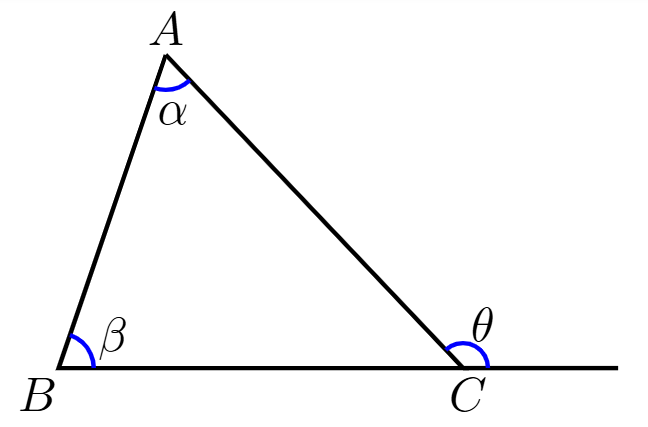
\includegraphics[height=4cm]{anglesint.png}
\end{figure}

\begin{proof}
    $\angle BCA = 180 - (\alpha + \beta)$ que implica el resultado 
    por el ángulo llano. 
\end{proof}

\section{... en Circunferencias}

Existen varios tipos de ángulos en circunferencias.

\begin{definition}[Ángulo central]
    Es el que tiene su vértice en el centro de un círculo y su 
    valor es igual al arco que interseca, es decir 
    $\alpha = arc(AB).$ 
\end{definition}

\begin{figure}[h]
    \centering
    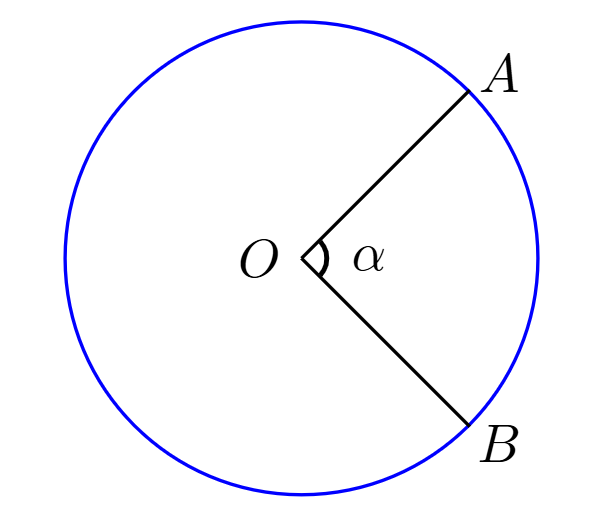
\includegraphics[height=4cm]{cangle.png}
\end{figure}

\begin{definition}[Ángulo inscrito]
    Es el que tiene su vértice sobre la circunferencia y su valor 
    es igual a la mitad del arco que interseca, es decir, 
    $\alpha = \frac{arc(AB)}{2}.$
\end{definition}

\begin{figure}[h]
    \centering
    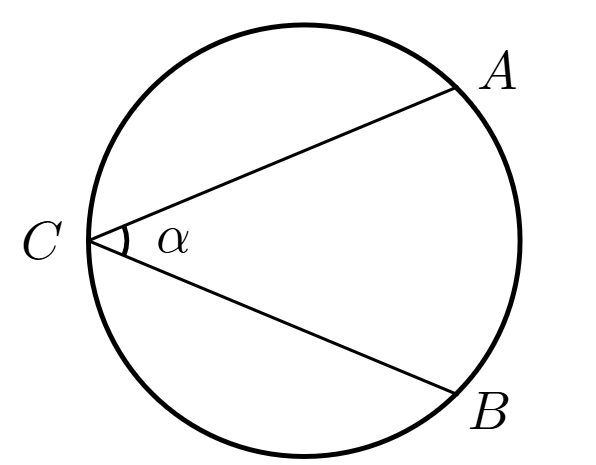
\includegraphics[height=4cm]{iangle.png}
\end{figure}

\begin{definition}[Ángulo sem-inscrito]
    Es el que tiene su vértice sobre la circunferencia y está 
    formado por una línea tangente y una secante. Su valor es igual 
    a la mitad del arco que interseca, es decir, 
    $\alpha = \frac{arc(AB)}{2}.$
\end{definition}

\begin{figure}[h]
    \centering
    \includegraphics[height=4cm]{sangle.png}
\end{figure}

\begin{theorem}
    El valor de un ángulo inscrito es igual a la mitad del ángulo 
    central que interseca el mismo arco.
\end{theorem}

\begin{figure}[h]
    \centering
    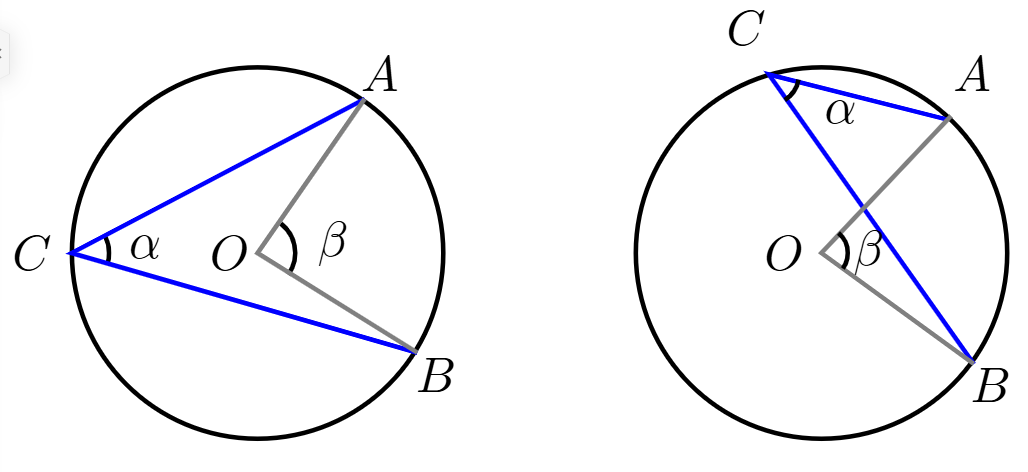
\includegraphics[height=4cm]{ciangle.png}
\end{figure}

\begin{theorem}[Ángulo interior]
    La magnitud del ángulo entre dos líneas que se cortan dentro
    de un círculo es equivalente a la semisuma de los arcos que 
    cortan dichas líneas. Es decir, 
    $\alpha = \frac{arc(AB)+arc{CD}}{2}.$
\end{theorem}

\begin{figure}[h]
    \centering
    \includegraphics[height=4cm]{intangle.png}
\end{figure}

\begin{proof}
    Ver figura.
\end{proof}

\begin{theorem}[Ángulo exterior]
    La magnitud del ángulo entre dos líneas que se cortan fuera
    de un círculo es equivalente a la semidiferencia de los arcos que 
    cortan dichas líneas. Es decir, 
    $\alpha = \frac{arc(AB)-arc(CD)}{2}.$
\end{theorem}
\begin{proof}
    Ver figura.
\end{proof}

\begin{figure}[h]
    \centering
    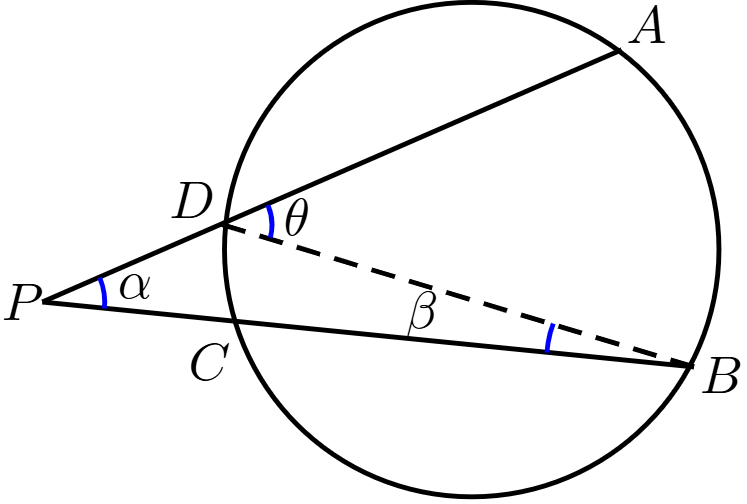
\includegraphics[height=4cm]{extangle.png}
\end{figure}

\subsection{Arsenal Adicional}

\begin{lemma}[Lema del Payaso]
    Para cualquier punto $P$ fuera de la circunferencia, si 
    $PA$ y $PB$ son tangentes $implies$ $\angle PAB = \angle PBA$, 
    $PA = PB$
\end{lemma}

\begin{figure}[h]
    \centering
    \includegraphics[height=4cm]{clown.png}
\end{figure}

\begin{proof}
    Al ser ángulos semi-inscritos que subtienden el mismo arco, 
    $\angle PAB = \angle PBA \implies \triangle PAB$ es isósceles, 
    dandonos la igualdad de lados que queríamos.
\end{proof}

\begin{lemma}
    El radio trazado hacia el punto de tangencia es perpendicular 
    a la tangente.
\end{lemma}

\begin{proof}
    La definición de ángulo semi-inscrito lo implica.
\end{proof}

\section{Bonus}

Los ángulos reciben nombres distintos dependiendo de su medida:

\begin{itemize}
    \item \textit{Agudo}: si es menor que \(90^\circ\).
    \item \textbf{Recto}: si es igual a \(90^\circ\).
    \item \textit{Obtuso}: si es mayor que \(90^\circ\) pero menor que \(180^\circ\).
    \item \textbf{Llano}: si es igual a \(180^\circ\).
    \item \textit{Cóncavo}: si es mayor que \(180^\circ\) pero menor que \(360^\circ\).
    \item \textit{Completo}: si es igual a \(360^\circ\).
\end{itemize}

Hay dos formas de clasificar a los triángulos: por sus lados o por sus ángulos.

Por sus ángulos, un triángulo puede ser:

\begin{itemize}
    \item \textit{Acutángulo}: si todos sus ángulos son agudos.
    \item \textbf{Rectángulo}: si tiene un ángulo recto.
    \item \textit{Obtusángulo}: si tiene un ángulo obtuso.
\end{itemize}

Por sus lados, un triángulo puede ser:

\begin{itemize}
    \item \textit{Escaleno}: si todos sus lados (por ende sus ángulos) son distintos.
    \item \textbf{Isósceles}: si hay una pareja de lados iguales. 
    Este tipo de triángulos también tiene una pareja de ángulos 
    iguales.
    \item \textbf{Equilátero}: si todos sus lados (por ende sus 
    ángulos) son iguales.
\end{itemize}

Nota que todos los triángulos equiláteros son isósceles.

\begin{definition}[Polígono regular]
    Aquel que tiene todos sus lados y ángulos iguales.
\end{definition}

\begin{definition}[Polígono convexo]
    Aquel que todos sus ángulos son menores a $180 \dg$.
\end{definition}

\begin{definition}[Polígono cóncavo]
    Aquel que tiene al menos un ángulo mayor a $180 \dg$.
\end{definition}

\newpage

\section{Problemas}

Cada problema que resuelvas te dará el número de treboles 
que especifica ($x \clubsuit$), ¡colecta los más que puedas!

\epigraph{Ya se la saben, angle chasing al fallo.}{Ransom, top en geo de México}

\begin{problem}[Gagos, $2 \clubsuit$]
    Encuentra el ángulo $x$.    
\end{problem}

\begin{figure}[!h]
    \centering
    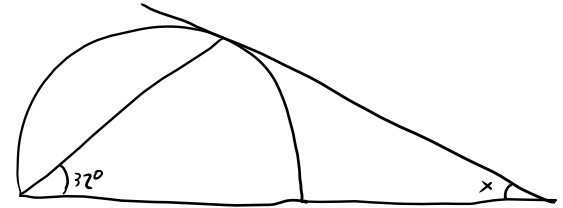
\includegraphics[height=2cm]{gagos1.png}
\end{figure}

\begin{problem}[Gagos, $2 \clubsuit$]
    Encuentra el ángulo $x$.    
\end{problem}

\begin{figure}[!h]
    \centering
    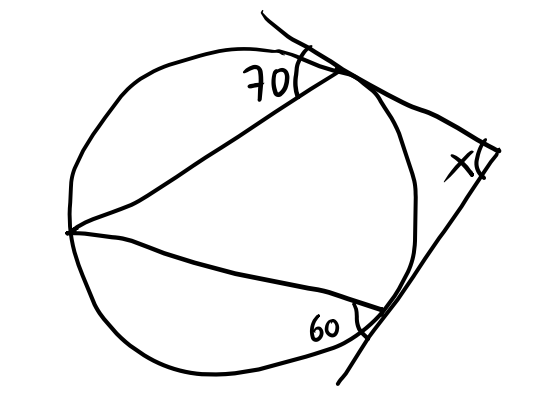
\includegraphics[height=3cm]{gagos2.png}
\end{figure}

\begin{problem}[$2 \clubsuit$]
    En el $\triangle ABC$, $\angle CAB + \angle ABC = 110 \dg$, y 
    $D$ es un punto sobre el segmento  $AB: CD = CB$ y $\angle DCA 
    = 10 \dg$. Calcula el valor del ángulo $\angle CAB$.
\end{problem}

\begin{figure}[!h]
    \centering
    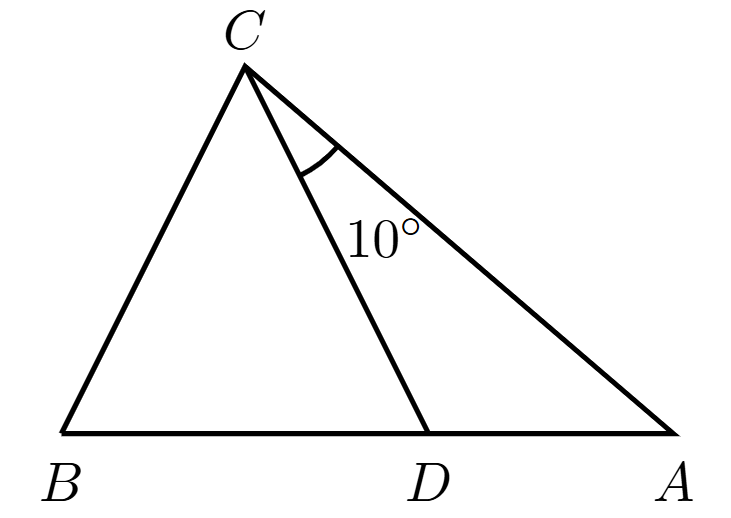
\includegraphics[height=3cm]{jjc1.png}
\end{figure}

\begin{sproblem}[$3 \clubsuit$]
    En la siguiente figura, ¿cuánto vale $a+b+c+d+e$?
\end{sproblem}

\begin{figure}[!h]
    \centering
    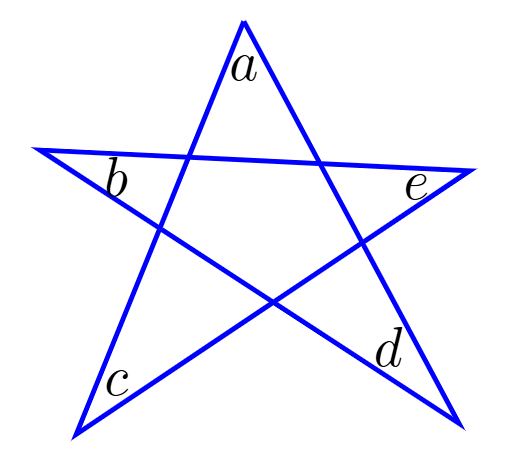
\includegraphics[height=4cm]{jjc2.png}
\end{figure}

\begin{problem}[$2 \clubsuit$]
    Encuentra cuanto vale $x$ en la siguiente figura.
\end{problem}

\begin{figure}[h!]
    \centering
    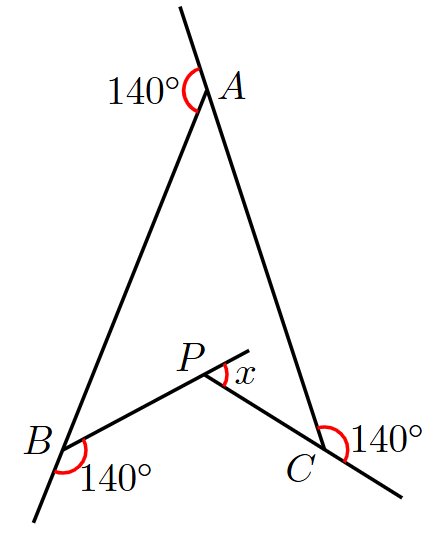
\includegraphics[height=4cm]{jjc3.png}
\end{figure}

\begin{problem}[$2 \clubsuit$]
    En la figura, los triángulos $\triangle PAB$, $\triangle PCD$ 
    son congruentes. Si $\angle APC = 67 \dg$ y $\angle CPD = 38 \dg$, 
    ¿cuánto mide $\angle BPC$ 
\end{problem}

\begin{figure}[h!]
    \centering
    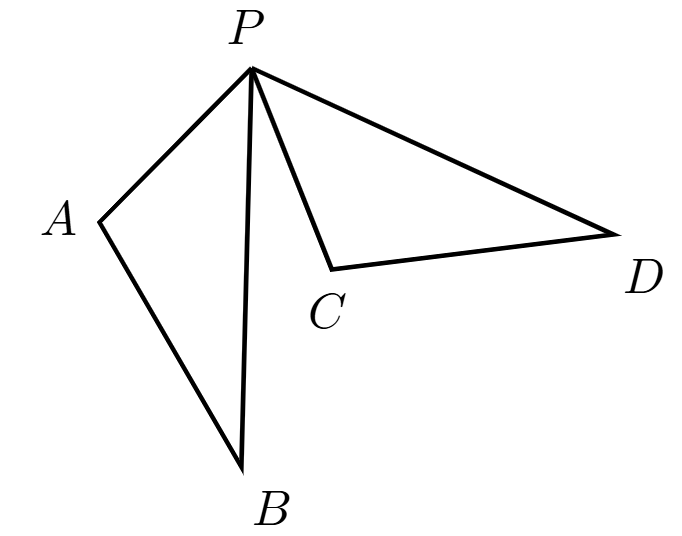
\includegraphics[height=4cm]{jjc4.png}
\end{figure}

\begin{problem}[OMMEB 2017, $3 \clubsuit$]
    En la siguiente figura, \(ABCDE\) es un pentágono regular 
    y \(ABFG\) es un cuadrado. ¿Cuál es la medida, en grados, 
    del ángulo \(GED\)?
\end{problem}

\begin{figure}[!h]
    \centering
    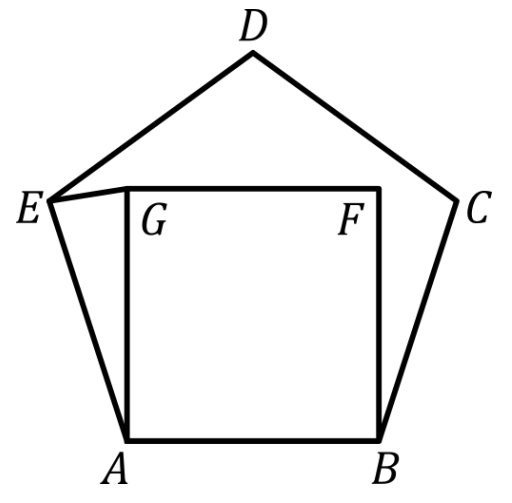
\includegraphics[height=3.5cm]{17OMMEBN1P8.png}
\end{figure}

\begin{problem}[OMMEB 2017, $3 \clubsuit$]
    En la siguiente figura, $ABCDEF$ es un hexágono regular y 
    $ABGHI$ es un pentágono regular. 
    ¿Cuál es la medida, en grados, del ángulo $IFE$?
\end{problem}

\begin{figure}[!h]
    \centering
    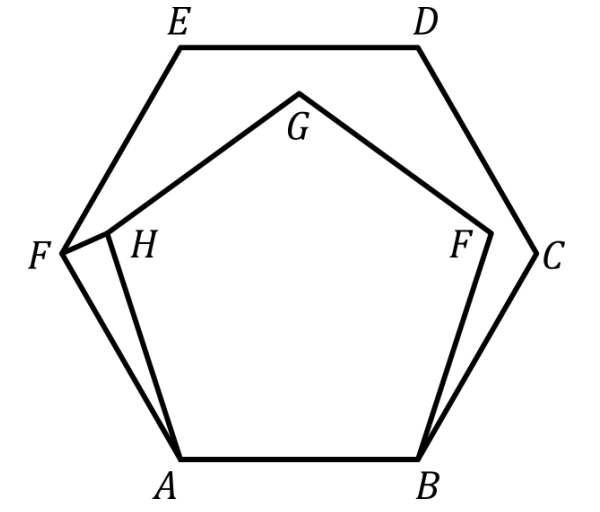
\includegraphics[height=3.5cm]{17OMMEBN2P3.png}
\end{figure}

\begin{problem}[Estatal 2024, $2 \clubsuit$]
    Sobre el cuadrado $ABCD$ se construyeron los triángulos 
    equiláteros $DCE$ y $ADF$. ¿Cuál es la medida del ángulo $x$?
\end{problem}
\begin{figure}[h!]
    \centering
    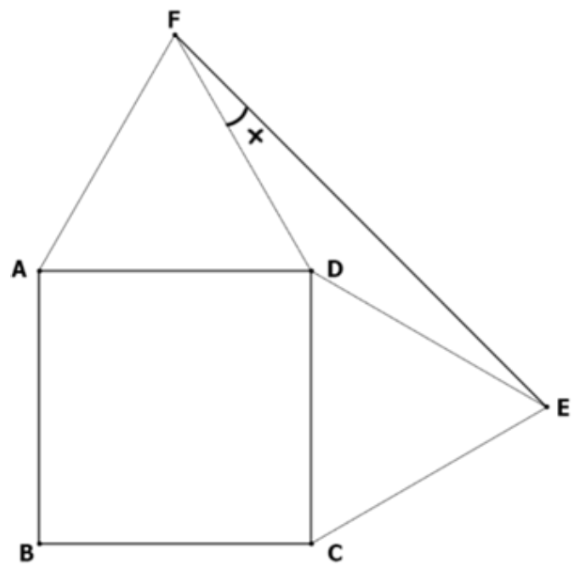
\includegraphics[height=4cm]{25ESTATAL1.png}
\end{figure}

\begin{problem}[Estatal 2025, $4 \clubsuit$]
    Dos cuadrados de distinto tamaño se dibujaron dentro de un 
    triángulo equilátero, como se muestra en la figura. ¿Cuánto 
    mide el ángulo marcado con $x$?
\end{problem}

\begin{figure}[h!]
    \centering
    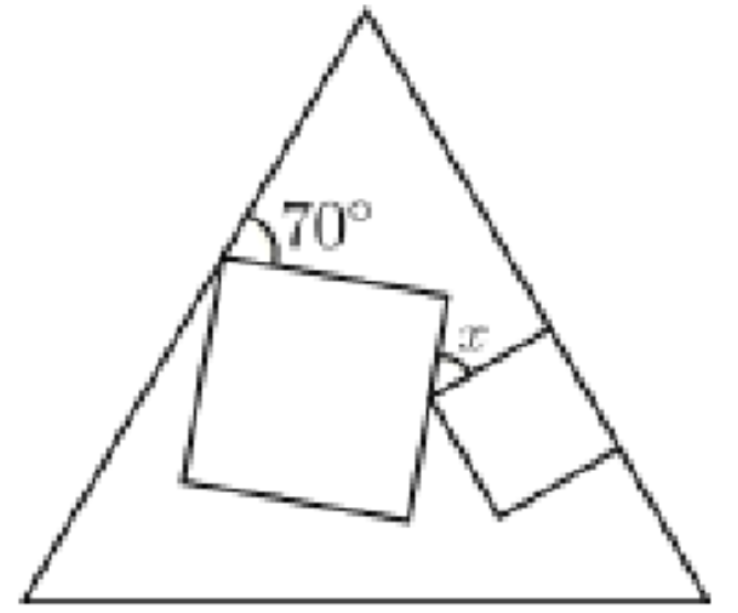
\includegraphics[height=3cm]{25ESTATAL4.png}
\end{figure}

\begin{problem}[Estatal 2025, $3 \clubsuit$]
    La siguiente figura está compuesta de dos pentágonos 
    regulares. Calcula la medida del ángulo $\angle FAD$.
\end{problem}

\begin{figure}[h!]
    \centering
    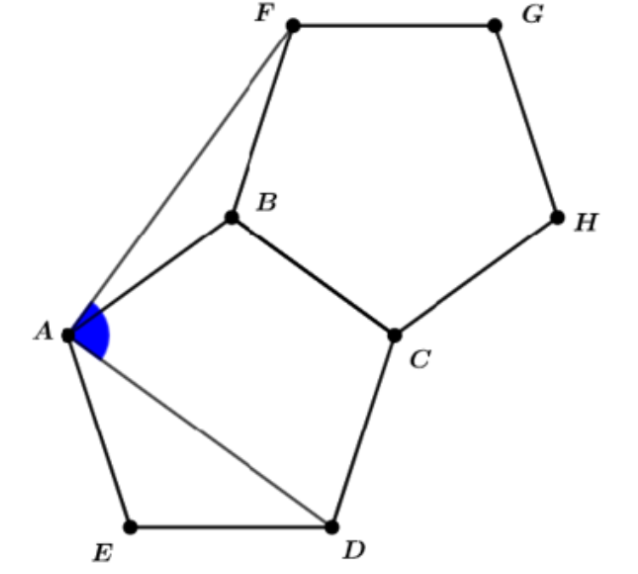
\includegraphics[height=4cm]{25ESTATAL3.png}
\end{figure}

\begin{problem}[Estatal 2025, $3 \clubsuit$]
    En la siguiente figura se muestra un cuadrilátero $ABCD$. 
    Si $BC=AD$, calcula la medida del ángulo $\angle ADC$.
\end{problem}

\begin{figure}[!h]
    \centering
    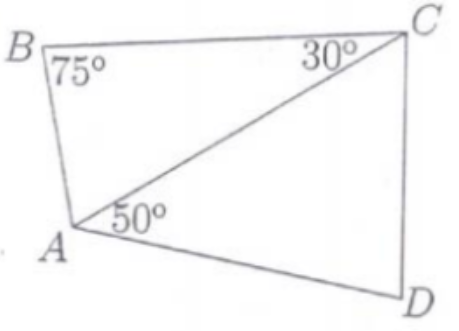
\includegraphics[height=3.5cm]{25ESTATAL7.png}
\end{figure}

\begin{dproblem}[Estatal 2024, $3 \clubsuit$]
    Encuentra el ángulo $x$.    
\end{dproblem}

\begin{figure}[!h]
    \centering
    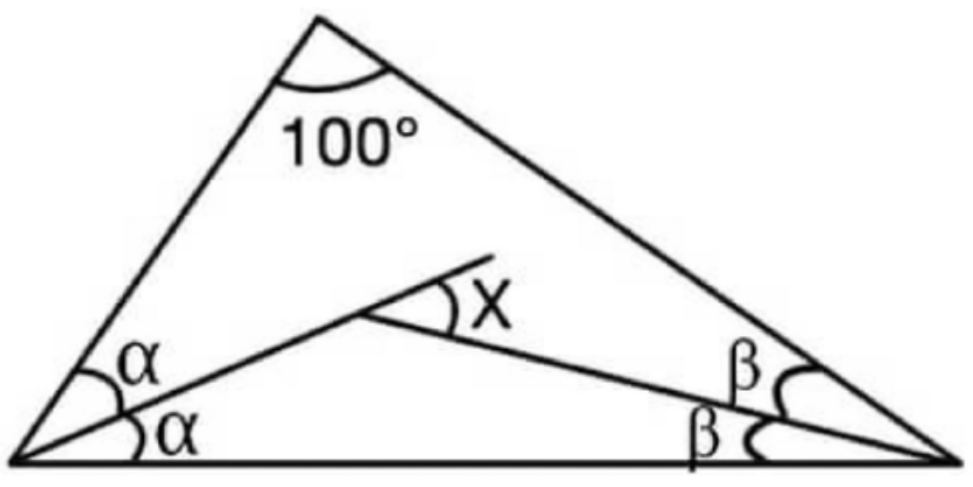
\includegraphics[height=3cm]{25ESTATAL2.png}
\end{figure}

\begin{problem}[$5 \clubsuit$]
    El trapecio isósceles $ABCD$ es tal que $AD = AB = BC = 1$ y 
    $DC = 2$, donde $AB \parallel DC$. ¿Cuánto mide $\angle CAD$?
\end{problem}

\begin{figure}[!h]
    \centering
    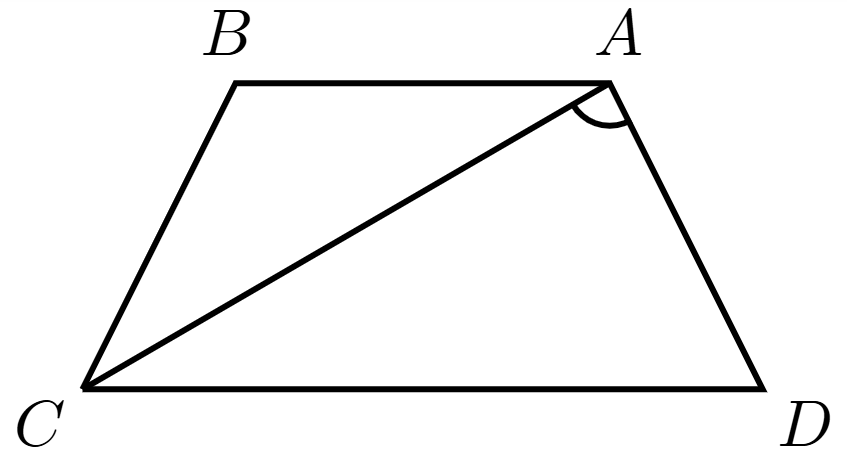
\includegraphics[height=3cm]{jjc5.png}
\end{figure}

\begin{remark}
    Un trapecio es un cuadrilátero con exactamente un par de 
    lados paralelos; es isósceles si sus dos lados no paralelos 
    son iguales.
\end{remark}


\begin{dproblem}[$3 \clubsuit$]
    Demuestra que dos líneas paralelas cualesquiera que intersecan
    una circunferencia, cortan arcos iguales entre ellas.
\end{dproblem}

\begin{dproblem}[$3 \clubsuit$]
    Uno de los lados de un triángulo inscrito en una 
    circunferencia coincide con un diámetro. Demuestra que el 
    triángulo es un triángulo rectángulo.
\end{dproblem}

\begin{dproblem}[$6 \clubsuit$]
    Demuestra que la razón entre la longitud del lado de un
    triángulo y el seno del ángulo opuesto es igual al diámetro 
    de la circunferencia que pasa por los tres vértices del triángulo.
\end{dproblem}

\begin{remark}
    Con eso, hemos demostrado que $\frac{a}{sin A} = 
    \frac{b}{sin B} = \frac{c}{sin C} = 2R$ que es conocido 
    como la \textit{Ley de Senos}.
\end{remark}

\begin{problem}[$4 \clubsuit$]
    Las circunferencias $C_1$ y $C_2$ se intersecan en los puntos 
    $A$y $B$. Se traza una recta $l$ qie corta a $C_1$ en 
    $C$ y $D$, y a $C_2$ en $M$ y $N$, de tal manera que $A$ y 
    $B$ quedan en distintos lados de $l$. Demuestra que $\angle 
    CAN + \angle MBD = 180 \dg$.
\end{problem}

\begin{problem}[$5 \clubsuit$]
    Demuestra que el valor de un ángulo semi-inscrito es igual 
    al valor de un ángulo inscrito que intersecte el mismo arco.
\end{problem}

\begin{problem}[$5 \clubsuit$]
    Una circunferencia ha sido dividida arbitrariamente en 
    cuatro partes, y los puntos medios de los arcos obtenidos se 
    han unido con segmentos de rectas. Demuestra que entre estos 
    segmentos dos serán perpendiculares entre sí.
\end{problem}

\begin{problem}[Estatal 2025, $5 \clubsuit$]
    En la figura, los puntos $A$,$P$,$Q$ y $R$ están sobre una 
    misma circunferencia con centro $C$, $ABCD$ es un cuadrado 
    de manera que $B$ y $D$ están sobre el segmento $PR$, además 
    $QR$ pasa por $C$. Determina el $\angle PQR$.
\end{problem}

\begin{figure}[!h]
    \centering
    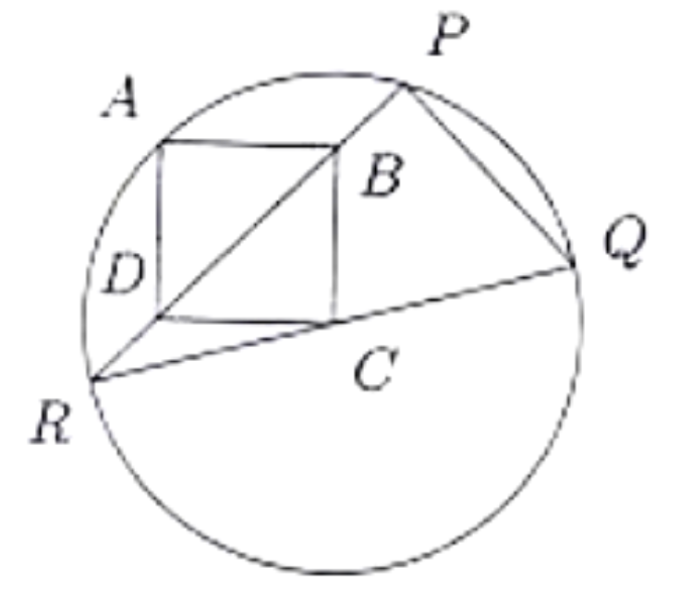
\includegraphics[height=3cm]{25ESTATAL6.png}
\end{figure}

\begin{problem}[$4 \clubsuit$]
    Dos circunferencias son tangentes exteriormente en un punto
    $A$. $BC$ es una tangente común externa. 
    Demuestra que $\angle BAC = 90 \dg$.
\end{problem}

\begin{problem}[$5 \clubsuit$]
    A una circunferencia se le han trazado dos líneas tangentes
    paralelas las cuales la tocan en los puntos $M$ y $N$. 
    Se traza una tercer tangente la cual corta a las tangentes 
    anteriores en los puntos $K$ y $L$. Sea $O$ el centro de la 
    circunferencia. Demuestra que $\angle KOL = 90\dg $.
\end{problem}

\begin{problem}[$6 \clubsuit$]
    Dos circunferencias se intersectan en los puntos $A$ y $B$ 
    como se muestra en la figura. Se escoge un punto arbitrario 
    $C$ en la primer circunferencia y se trazan los rayos $CA$ 
    y $CB$, los cuales intersectan la segunda circunferencia
    de nuevo en los puntos $D$ y $E$, respectivamente. Demuestra 
    que la longitud del segmento $DE$ no depende de la elección 
    del punto $C$.
\end{problem}

\begin{problem}[$4 \clubsuit$]
    Dos circunferencias de centros $O_1$ y $O_2$ se intersectan 
    en los puntos $A$ y $B$, como se muestra en la figura. La 
    línea $CD$ es tangente a ambas circunferencias. Demuestra que
    $\angle CAD = \half \angle O_1AO_2$
\end{problem}

\begin{figure}[!h]
    \centering
    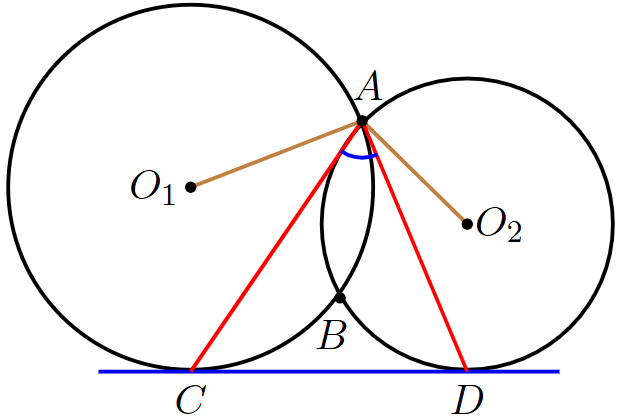
\includegraphics[height=3cm]{jjc6.png}
\end{figure}

\begin{problem}[$7 \clubsuit$]
    Sea ABCD un cuadrilátero cíclico. Las líneas AB y DC se 
    intersecan en un punto $Q$ y las líneas $DA$ y $CB$ en 
    un punto $Q$. Demuestra que las líneas que bisecan los 
    ángulos $\angle DPC$ y $\angle AQD$ son perpendiculares.
\end{problem}

\begin{remark}
    Un cuadrilátero es cíclico si existe una circunferencia que 
    pasa por sus cuatro vértices. Bisecar significa dividir 
    en dos partes iguales.
\end{remark}

\noindent El máximo número de $\clubsuit$ en este capítulo es de 
$96 \clubsuit$.
